% Options for packages loaded elsewhere
\PassOptionsToPackage{unicode}{hyperref}
\PassOptionsToPackage{hyphens}{url}
\PassOptionsToPackage{dvipsnames,svgnames,x11names}{xcolor}
%
\documentclass[
  letterpaper,
  DIV=11,
  numbers=noendperiod]{scrartcl}

\usepackage{amsmath,amssymb}
\usepackage{lmodern}
\usepackage{iftex}
\ifPDFTeX
  \usepackage[T1]{fontenc}
  \usepackage[utf8]{inputenc}
  \usepackage{textcomp} % provide euro and other symbols
\else % if luatex or xetex
  \usepackage{unicode-math}
  \defaultfontfeatures{Scale=MatchLowercase}
  \defaultfontfeatures[\rmfamily]{Ligatures=TeX,Scale=1}
\fi
% Use upquote if available, for straight quotes in verbatim environments
\IfFileExists{upquote.sty}{\usepackage{upquote}}{}
\IfFileExists{microtype.sty}{% use microtype if available
  \usepackage[]{microtype}
  \UseMicrotypeSet[protrusion]{basicmath} % disable protrusion for tt fonts
}{}
\makeatletter
\@ifundefined{KOMAClassName}{% if non-KOMA class
  \IfFileExists{parskip.sty}{%
    \usepackage{parskip}
  }{% else
    \setlength{\parindent}{0pt}
    \setlength{\parskip}{6pt plus 2pt minus 1pt}}
}{% if KOMA class
  \KOMAoptions{parskip=half}}
\makeatother
\usepackage{xcolor}
\setlength{\emergencystretch}{3em} % prevent overfull lines
\setcounter{secnumdepth}{-\maxdimen} % remove section numbering
% Make \paragraph and \subparagraph free-standing
\ifx\paragraph\undefined\else
  \let\oldparagraph\paragraph
  \renewcommand{\paragraph}[1]{\oldparagraph{#1}\mbox{}}
\fi
\ifx\subparagraph\undefined\else
  \let\oldsubparagraph\subparagraph
  \renewcommand{\subparagraph}[1]{\oldsubparagraph{#1}\mbox{}}
\fi

\usepackage{color}
\usepackage{fancyvrb}
\newcommand{\VerbBar}{|}
\newcommand{\VERB}{\Verb[commandchars=\\\{\}]}
\DefineVerbatimEnvironment{Highlighting}{Verbatim}{commandchars=\\\{\}}
% Add ',fontsize=\small' for more characters per line
\usepackage{framed}
\definecolor{shadecolor}{RGB}{241,243,245}
\newenvironment{Shaded}{\begin{snugshade}}{\end{snugshade}}
\newcommand{\AlertTok}[1]{\textcolor[rgb]{0.68,0.00,0.00}{#1}}
\newcommand{\AnnotationTok}[1]{\textcolor[rgb]{0.37,0.37,0.37}{#1}}
\newcommand{\AttributeTok}[1]{\textcolor[rgb]{0.40,0.45,0.13}{#1}}
\newcommand{\BaseNTok}[1]{\textcolor[rgb]{0.68,0.00,0.00}{#1}}
\newcommand{\BuiltInTok}[1]{\textcolor[rgb]{0.00,0.23,0.31}{#1}}
\newcommand{\CharTok}[1]{\textcolor[rgb]{0.13,0.47,0.30}{#1}}
\newcommand{\CommentTok}[1]{\textcolor[rgb]{0.37,0.37,0.37}{#1}}
\newcommand{\CommentVarTok}[1]{\textcolor[rgb]{0.37,0.37,0.37}{\textit{#1}}}
\newcommand{\ConstantTok}[1]{\textcolor[rgb]{0.56,0.35,0.01}{#1}}
\newcommand{\ControlFlowTok}[1]{\textcolor[rgb]{0.00,0.23,0.31}{#1}}
\newcommand{\DataTypeTok}[1]{\textcolor[rgb]{0.68,0.00,0.00}{#1}}
\newcommand{\DecValTok}[1]{\textcolor[rgb]{0.68,0.00,0.00}{#1}}
\newcommand{\DocumentationTok}[1]{\textcolor[rgb]{0.37,0.37,0.37}{\textit{#1}}}
\newcommand{\ErrorTok}[1]{\textcolor[rgb]{0.68,0.00,0.00}{#1}}
\newcommand{\ExtensionTok}[1]{\textcolor[rgb]{0.00,0.23,0.31}{#1}}
\newcommand{\FloatTok}[1]{\textcolor[rgb]{0.68,0.00,0.00}{#1}}
\newcommand{\FunctionTok}[1]{\textcolor[rgb]{0.28,0.35,0.67}{#1}}
\newcommand{\ImportTok}[1]{\textcolor[rgb]{0.00,0.46,0.62}{#1}}
\newcommand{\InformationTok}[1]{\textcolor[rgb]{0.37,0.37,0.37}{#1}}
\newcommand{\KeywordTok}[1]{\textcolor[rgb]{0.00,0.23,0.31}{#1}}
\newcommand{\NormalTok}[1]{\textcolor[rgb]{0.00,0.23,0.31}{#1}}
\newcommand{\OperatorTok}[1]{\textcolor[rgb]{0.37,0.37,0.37}{#1}}
\newcommand{\OtherTok}[1]{\textcolor[rgb]{0.00,0.23,0.31}{#1}}
\newcommand{\PreprocessorTok}[1]{\textcolor[rgb]{0.68,0.00,0.00}{#1}}
\newcommand{\RegionMarkerTok}[1]{\textcolor[rgb]{0.00,0.23,0.31}{#1}}
\newcommand{\SpecialCharTok}[1]{\textcolor[rgb]{0.37,0.37,0.37}{#1}}
\newcommand{\SpecialStringTok}[1]{\textcolor[rgb]{0.13,0.47,0.30}{#1}}
\newcommand{\StringTok}[1]{\textcolor[rgb]{0.13,0.47,0.30}{#1}}
\newcommand{\VariableTok}[1]{\textcolor[rgb]{0.07,0.07,0.07}{#1}}
\newcommand{\VerbatimStringTok}[1]{\textcolor[rgb]{0.13,0.47,0.30}{#1}}
\newcommand{\WarningTok}[1]{\textcolor[rgb]{0.37,0.37,0.37}{\textit{#1}}}

\providecommand{\tightlist}{%
  \setlength{\itemsep}{0pt}\setlength{\parskip}{0pt}}\usepackage{longtable,booktabs,array}
\usepackage{calc} % for calculating minipage widths
% Correct order of tables after \paragraph or \subparagraph
\usepackage{etoolbox}
\makeatletter
\patchcmd\longtable{\par}{\if@noskipsec\mbox{}\fi\par}{}{}
\makeatother
% Allow footnotes in longtable head/foot
\IfFileExists{footnotehyper.sty}{\usepackage{footnotehyper}}{\usepackage{footnote}}
\makesavenoteenv{longtable}
\usepackage{graphicx}
\makeatletter
\def\maxwidth{\ifdim\Gin@nat@width>\linewidth\linewidth\else\Gin@nat@width\fi}
\def\maxheight{\ifdim\Gin@nat@height>\textheight\textheight\else\Gin@nat@height\fi}
\makeatother
% Scale images if necessary, so that they will not overflow the page
% margins by default, and it is still possible to overwrite the defaults
% using explicit options in \includegraphics[width, height, ...]{}
\setkeys{Gin}{width=\maxwidth,height=\maxheight,keepaspectratio}
% Set default figure placement to htbp
\makeatletter
\def\fps@figure{htbp}
\makeatother
\newlength{\cslhangindent}
\setlength{\cslhangindent}{1.5em}
\newlength{\csllabelwidth}
\setlength{\csllabelwidth}{3em}
\newlength{\cslentryspacingunit} % times entry-spacing
\setlength{\cslentryspacingunit}{\parskip}
\newenvironment{CSLReferences}[2] % #1 hanging-ident, #2 entry spacing
 {% don't indent paragraphs
  \setlength{\parindent}{0pt}
  % turn on hanging indent if param 1 is 1
  \ifodd #1
  \let\oldpar\par
  \def\par{\hangindent=\cslhangindent\oldpar}
  \fi
  % set entry spacing
  \setlength{\parskip}{#2\cslentryspacingunit}
 }%
 {}
\usepackage{calc}
\newcommand{\CSLBlock}[1]{#1\hfill\break}
\newcommand{\CSLLeftMargin}[1]{\parbox[t]{\csllabelwidth}{#1}}
\newcommand{\CSLRightInline}[1]{\parbox[t]{\linewidth - \csllabelwidth}{#1}\break}
\newcommand{\CSLIndent}[1]{\hspace{\cslhangindent}#1}

\KOMAoption{captions}{tableheading}
\makeatletter
\@ifpackageloaded{tcolorbox}{}{\usepackage[many]{tcolorbox}}
\@ifpackageloaded{fontawesome5}{}{\usepackage{fontawesome5}}
\definecolor{quarto-callout-color}{HTML}{909090}
\definecolor{quarto-callout-note-color}{HTML}{0758E5}
\definecolor{quarto-callout-important-color}{HTML}{CC1914}
\definecolor{quarto-callout-warning-color}{HTML}{EB9113}
\definecolor{quarto-callout-tip-color}{HTML}{00A047}
\definecolor{quarto-callout-caution-color}{HTML}{FC5300}
\definecolor{quarto-callout-color-frame}{HTML}{acacac}
\definecolor{quarto-callout-note-color-frame}{HTML}{4582ec}
\definecolor{quarto-callout-important-color-frame}{HTML}{d9534f}
\definecolor{quarto-callout-warning-color-frame}{HTML}{f0ad4e}
\definecolor{quarto-callout-tip-color-frame}{HTML}{02b875}
\definecolor{quarto-callout-caution-color-frame}{HTML}{fd7e14}
\makeatother
\makeatletter
\makeatother
\makeatletter
\makeatother
\makeatletter
\@ifpackageloaded{caption}{}{\usepackage{caption}}
\AtBeginDocument{%
\ifdefined\contentsname
  \renewcommand*\contentsname{Table of contents}
\else
  \newcommand\contentsname{Table of contents}
\fi
\ifdefined\listfigurename
  \renewcommand*\listfigurename{List of Figures}
\else
  \newcommand\listfigurename{List of Figures}
\fi
\ifdefined\listtablename
  \renewcommand*\listtablename{List of Tables}
\else
  \newcommand\listtablename{List of Tables}
\fi
\ifdefined\figurename
  \renewcommand*\figurename{Figure}
\else
  \newcommand\figurename{Figure}
\fi
\ifdefined\tablename
  \renewcommand*\tablename{Table}
\else
  \newcommand\tablename{Table}
\fi
}
\@ifpackageloaded{float}{}{\usepackage{float}}
\floatstyle{ruled}
\@ifundefined{c@chapter}{\newfloat{codelisting}{h}{lop}}{\newfloat{codelisting}{h}{lop}[chapter]}
\floatname{codelisting}{Listing}
\newcommand*\listoflistings{\listof{codelisting}{List of Listings}}
\makeatother
\makeatletter
\@ifpackageloaded{caption}{}{\usepackage{caption}}
\@ifpackageloaded{subcaption}{}{\usepackage{subcaption}}
\makeatother
\makeatletter
\@ifpackageloaded{tcolorbox}{}{\usepackage[many]{tcolorbox}}
\makeatother
\makeatletter
\@ifundefined{shadecolor}{\definecolor{shadecolor}{rgb}{.97, .97, .97}}
\makeatother
\makeatletter
\makeatother
\ifLuaTeX
  \usepackage{selnolig}  % disable illegal ligatures
\fi
\IfFileExists{bookmark.sty}{\usepackage{bookmark}}{\usepackage{hyperref}}
\IfFileExists{xurl.sty}{\usepackage{xurl}}{} % add URL line breaks if available
\urlstyle{same} % disable monospaced font for URLs
\hypersetup{
  pdftitle={Homework 2},
  pdfauthor={Shao-Ting Chiu (UIN:433002162)},
  colorlinks=true,
  linkcolor={blue},
  filecolor={Maroon},
  citecolor={Blue},
  urlcolor={Blue},
  pdfcreator={LaTeX via pandoc}}

\title{Homework 2}
\author{Shao-Ting Chiu (UIN:433002162)}
\date{10/6/22}

\begin{document}
\maketitle
\ifdefined\Shaded\renewenvironment{Shaded}{\begin{tcolorbox}[frame hidden, boxrule=0pt, borderline west={3pt}{0pt}{shadecolor}, interior hidden, enhanced, breakable, sharp corners]}{\end{tcolorbox}}\fi

\renewcommand*\contentsname{Table of contents}
{
\hypersetup{linkcolor=}
\setcounter{tocdepth}{3}
\tableofcontents
}
\hypertarget{homework-description}{%
\subsection{Homework Description}\label{homework-description}}

\begin{itemize}
\tightlist
\item
  Course: ECEN649, Fall2022
\end{itemize}

\begin{quote}
Problems from the book:

3.6 (10 pt)

4.2 (10 pt)

4.3 (10 pt)

4.4 (10 pt)

4.8 (20 pt)
\end{quote}

\begin{itemize}
\tightlist
\item
  Deadline: \texttt{Oct.\ 12th,\ 11:59\ am}
\end{itemize}

\hypertarget{computational-enviromnent-setup}{%
\subsection{Computational Enviromnent
Setup}\label{computational-enviromnent-setup}}

\hypertarget{third-party-libraries}\NormalTok{matplotlib inline}
\ImportTok{import}\NormalTok{ sys }\CommentTok{\# system information}
\ImportTok{import}\NormalTok{ matplotlib }\CommentTok{\# plotting}
\ImportTok{import}\NormalTok{ scipy.stats }\ImportTok{as}\NormalTok{ st }\CommentTok{\# scientific computing}
\ImportTok{import}\NormalTok{ pandas }\ImportTok{as}\NormalTok{ pd }\CommentTok{\# data managing}
\ImportTok{import}\NormalTok{ numpy }\ImportTok{as}\NormalTok{ np }\CommentTok{\# numerical comuptation}
\ImportTok{from}\NormalTok{ numpy }\ImportTok{import}\NormalTok{ linalg }\ImportTok{as}\NormalTok{ LA}
\ImportTok{import}\NormalTok{ scipy }\ImportTok{as}\NormalTok{ sp}
\ImportTok{import}\NormalTok{ scipy.optimize }\ImportTok{as}\NormalTok{ opt}
\ImportTok{import}\NormalTok{ sympy }\ImportTok{as}\NormalTok{ sp}
\ImportTok{import}\NormalTok{ matplotlib.pyplot }\ImportTok{as}\NormalTok{ plt}
\ImportTok{from}\NormalTok{ numpy.linalg }\ImportTok{import}\NormalTok{ inv, det}
\ImportTok{from}\NormalTok{ numpy.random }\ImportTok{import}\NormalTok{ multivariate\_normal }\ImportTok{as}\NormalTok{ mvn}
\ImportTok{from}\NormalTok{ numpy.random }\ImportTok{import}\NormalTok{ binomial }\ImportTok{as}\NormalTok{ binom}
\CommentTok{\# Matplotlib setting}
\NormalTok{plt.rcParams[}\StringTok{\textquotesingle{}text.usetex\textquotesingle{}}\NormalTok{] }\OperatorTok{=} \VariableTok{True}
\NormalTok{matplotlib.rcParams[}\StringTok{\textquotesingle{}figure.dpi\textquotesingle{}}\NormalTok{]}\OperatorTok{=} \DecValTok{300}
\end{Highlighting}
\end{Shaded}

\hypertarget{version}{%
\subsubsection{Version}\label{version}}

\begin{Shaded}
\begin{Highlighting}[numbers=left,,]
\BuiltInTok{print}\NormalTok{(sys.version)}
\BuiltInTok{print}\NormalTok{(matplotlib.\_\_version\_\_)}
\BuiltInTok{print}\NormalTok{(sp.\_\_version\_\_)}
\BuiltInTok{print}\NormalTok{(np.\_\_version\_\_)}
\BuiltInTok{print}\NormalTok{(pd.\_\_version\_\_)}
\end{Highlighting}
\end{Shaded}

\begin{verbatim}
3.8.12 (default, Oct 22 2021, 18:39:35) 
[Clang 13.0.0 (clang-1300.0.29.3)]
3.3.1
1.6.2
1.19.1
1.1.1
\end{verbatim}

\begin{center}\rule{0.5\linewidth}{0.5pt}\end{center}

\hypertarget{problem-3.6-python-assignment}{%
\subsection{Problem 3.6 (Python
Assignment)}\label{problem-3.6-python-assignment}}

\begin{quote}
Using the synthetic data model in Section A8.1 for the homoskedastic
case with \(\mu_0 = (0,\dots,0)\), \(\mu_1=(1,\dots,1)\),
\(P(Y=0)=P(Y=1)\), and \(k=d\) (independent features), generate a large
number (e.g., \(M=1000\)) of training data sets for each sample size
\(n=20\) to \(n=100\), in steps of \(10\), with \(d=2,5,8\), and
\(\sigma=1\). Obtain an approximation of the expected classification
error \(E[\epsilon_n]\) of the nearest centroid classifier in each case
by averaging \(\epsilon_n\), computed using the exact formula (3.13),
over the \(M\) synthetic training data sets. Plot \(E[\epsilon_n]\) as a
function of the sample size, for \(d=2,5,8\) (join the individual points
with lines to obtain a smooth curve). Explain what you see.
\end{quote}

\begin{itemize}
\tightlist
\item
  The formula in Braga-Neto (2020, 56, Eq. 3.13)

  \begin{itemize}
  \tightlist
  \item
    \(\epsilon_n = \frac{1}{2}\left(\Phi\left(\frac{a_{n}^{T}\hat{\mu}_0 + b_n}{\|a_n\|}\right) + \Phi\left(-\frac{a_{n}^{T}\hat{\mu}_1 + b_n}{\|a_n\|}\right) \right)\)

    \begin{itemize}
    \tightlist
    \item
      \(\mu_0 = (0,\dots, 0)\)
      \(\hat{\mu}_0 = \frac{1}{N_0}\sum^{n}_{i=1}X_i I_{Y_i=0}\)
    \item
      \(\mu_1 = (1,\dots,1)\)
      \(\hat{\mu}_1 = \frac{1}{N_1}\sum^{n}_{i=1}X_i I_{Y_i=1}\)
    \item
      \(a_n = \hat{\mu}_1 - \hat{\mu}_0\)
    \item
      \(b_n = \frac{(\hat{\mu}_1 - \hat{\mu}_0)(\hat{\mu}_1 + \hat{\mu}_0)}{2}\)
    \end{itemize}
  \end{itemize}
\end{itemize}

\begin{Shaded}
\begin{Highlighting}[numbers=left,,]
\KeywordTok{def}\NormalTok{ hat\_mu(m):}
    \ControlFlowTok{return}\NormalTok{ np.mean(m, axis}\OperatorTok{=}\DecValTok{0}\NormalTok{)}

\KeywordTok{def}\NormalTok{ get\_an(hm0,hm1):}
    \ControlFlowTok{return}\NormalTok{ hm1 }\OperatorTok{{-}}\NormalTok{ hm0}

\KeywordTok{def}\NormalTok{ get\_bn(hm0,hm1):}
    \ControlFlowTok{return}\NormalTok{ (hm1 }\OperatorTok{{-}}\NormalTok{ hm0)}\OperatorTok{*}\NormalTok{(hm1}\OperatorTok{+}\NormalTok{hm0).T}\OperatorTok{/}\DecValTok{2}

\KeywordTok{def}\NormalTok{ epsilon(hmu0, hmu1, p0}\OperatorTok{=}\FloatTok{0.5}\NormalTok{):}
\NormalTok{    p1 }\OperatorTok{=} \DecValTok{1}\OperatorTok{{-}}\NormalTok{p0}
\NormalTok{    an }\OperatorTok{=}\NormalTok{ get\_an(hmu0, hmu1)}
\NormalTok{    bn }\OperatorTok{=}\NormalTok{ get\_bn(hmu0, hmu1)}
\NormalTok{    epsilon0 }\OperatorTok{=}\NormalTok{ st.norm.cdf((an}\OperatorTok{*}\NormalTok{hmu0.T }\OperatorTok{+}\NormalTok{ bn)}\OperatorTok{/}\NormalTok{LA.norm(an))}
\NormalTok{    epsilon1 }\OperatorTok{=}\NormalTok{ st.norm.cdf(}\OperatorTok{{-}}\NormalTok{(an}\OperatorTok{*}\NormalTok{hmu1.T}\OperatorTok{+}\NormalTok{ bn)}\OperatorTok{/}\NormalTok{LA.norm(an))}
    \ControlFlowTok{return}\NormalTok{ (p0}\OperatorTok{*}\NormalTok{epsilon0 }\OperatorTok{+}\NormalTok{ p1}\OperatorTok{*}\NormalTok{epsilon1)[}\DecValTok{0}\NormalTok{][}\DecValTok{0}\NormalTok{]}

\KeywordTok{class}\NormalTok{ GaussianDataGen:}
    \KeywordTok{def} \FunctionTok{\_\_init\_\_}\NormalTok{(}\VariableTok{self}\NormalTok{, n, d, s}\OperatorTok{=}\DecValTok{1}\NormalTok{, mu}\OperatorTok{=}\DecValTok{0}\NormalTok{):}
        \VariableTok{self}\NormalTok{.n }\OperatorTok{=}\NormalTok{ n}
        \VariableTok{self}\NormalTok{.d }\OperatorTok{=}\NormalTok{ d}
        \VariableTok{self}\NormalTok{.mu }\OperatorTok{=}\NormalTok{ np.ones(d) }\OperatorTok{*}\NormalTok{ mu}
        \VariableTok{self}\NormalTok{.s }\OperatorTok{=}\NormalTok{ s}
        \VariableTok{self}\NormalTok{.cov }\OperatorTok{=} \VariableTok{self}\NormalTok{.get\_cov()}

    \KeywordTok{def}\NormalTok{ get\_cov(}\VariableTok{self}\NormalTok{):}
        \ControlFlowTok{return}\NormalTok{ np.identity(}\VariableTok{self}\NormalTok{.d) }\OperatorTok{*} \VariableTok{self}\NormalTok{.s}
    
    \KeywordTok{def}\NormalTok{ sample(}\VariableTok{self}\NormalTok{):}
\NormalTok{        hmuV }\OperatorTok{=}\NormalTok{ np.zeros(}\VariableTok{self}\NormalTok{.d)}
        \ControlFlowTok{for}\NormalTok{ i }\KeywordTok{in} \BuiltInTok{range}\NormalTok{(}\DecValTok{0}\NormalTok{,}\VariableTok{self}\NormalTok{.d):}
\NormalTok{            hmuV[i] }\OperatorTok{=}\NormalTok{ np.mean(np.random.normal(}\VariableTok{self}\NormalTok{.mu[}\DecValTok{0}\NormalTok{], }\VariableTok{self}\NormalTok{.s, }\VariableTok{self}\NormalTok{.n))}
        \ControlFlowTok{return}\NormalTok{ np.matrix(hmuV)}

\KeywordTok{def}\NormalTok{ cal\_eps(dg0, dg1, p0}\OperatorTok{=}\FloatTok{0.5}\NormalTok{):}
\NormalTok{    hmuV0 }\OperatorTok{=}\NormalTok{ dg0.sample()}
\NormalTok{    hmuV1 }\OperatorTok{=}\NormalTok{ dg1.sample()}
    \ControlFlowTok{return}\NormalTok{ epsilon(hmuV0, hmuV1, p0}\OperatorTok{=}\FloatTok{0.5}\NormalTok{)}
\NormalTok{cal\_eps\_func }\OperatorTok{=}\NormalTok{ np.vectorize(cal\_eps)}

\KeywordTok{def}\NormalTok{ exp\_try\_nd(n, d, s}\OperatorTok{=}\DecValTok{1}\NormalTok{,M}\OperatorTok{=}\DecValTok{1000}\NormalTok{):}
\NormalTok{    gX0 }\OperatorTok{=}\NormalTok{ GaussianDataGen(n}\OperatorTok{=}\NormalTok{n, d}\OperatorTok{=}\NormalTok{d, s}\OperatorTok{=}\NormalTok{ s,mu}\OperatorTok{=}\DecValTok{0}\NormalTok{)}
\NormalTok{    gX1 }\OperatorTok{=}\NormalTok{ GaussianDataGen(n}\OperatorTok{=}\NormalTok{n, d}\OperatorTok{=}\NormalTok{d, s}\OperatorTok{=}\NormalTok{ s, mu}\OperatorTok{=}\DecValTok{1}\NormalTok{)}
\NormalTok{    eps }\OperatorTok{=}\NormalTok{ cal\_eps\_func([gX0 }\ControlFlowTok{for}\NormalTok{ i }\KeywordTok{in} \BuiltInTok{range}\NormalTok{(}\DecValTok{0}\NormalTok{,M)], gX1)}
    \ControlFlowTok{return}\NormalTok{ np.mean(eps)}
\NormalTok{exp\_try\_nd\_func }\OperatorTok{=}\NormalTok{ np.vectorize(exp\_try\_nd)}

\NormalTok{M }\OperatorTok{=} \DecValTok{1000}
\NormalTok{ns }\OperatorTok{=}\NormalTok{ np.arange(}\DecValTok{20}\NormalTok{,}\DecValTok{80}\NormalTok{, }\DecValTok{10}\NormalTok{)}
\NormalTok{s }\OperatorTok{=} \DecValTok{1}
\NormalTok{dres }\OperatorTok{=}\NormalTok{ \{}\DecValTok{2}\NormalTok{:[],}\DecValTok{5}\NormalTok{:[],}\DecValTok{8}\NormalTok{:[]\}}


\ControlFlowTok{for}\NormalTok{ k }\KeywordTok{in}\NormalTok{ dres.keys():}
\NormalTok{    dres[k] }\OperatorTok{=}\NormalTok{ exp\_try\_nd\_func(ns,k,M)}


\NormalTok{fig, ax }\OperatorTok{=}\NormalTok{ plt.subplots()}
\ControlFlowTok{for}\NormalTok{ k }\KeywordTok{in}\NormalTok{ dres.keys():}
\NormalTok{    ax.plot(ns, dres[k], }\StringTok{\textquotesingle{}o\textquotesingle{}}\NormalTok{,label}\OperatorTok{=}\StringTok{"d=}\SpecialCharTok{\{\}}\StringTok{"}\NormalTok{.}\BuiltInTok{format}\NormalTok{(k))}
\NormalTok{ax.set\_xlabel(}\StringTok{"n"}\NormalTok{)}
\NormalTok{ax.set\_ylabel(}\StringTok{"$E[}\CharTok{\textbackslash{}\textbackslash{}}\StringTok{epsilon\_n]$"}\NormalTok{)}
\NormalTok{ax.legend()}\OperatorTok{;}
\end{Highlighting}
\end{Shaded}

\begin{figure}[H]

{\centering 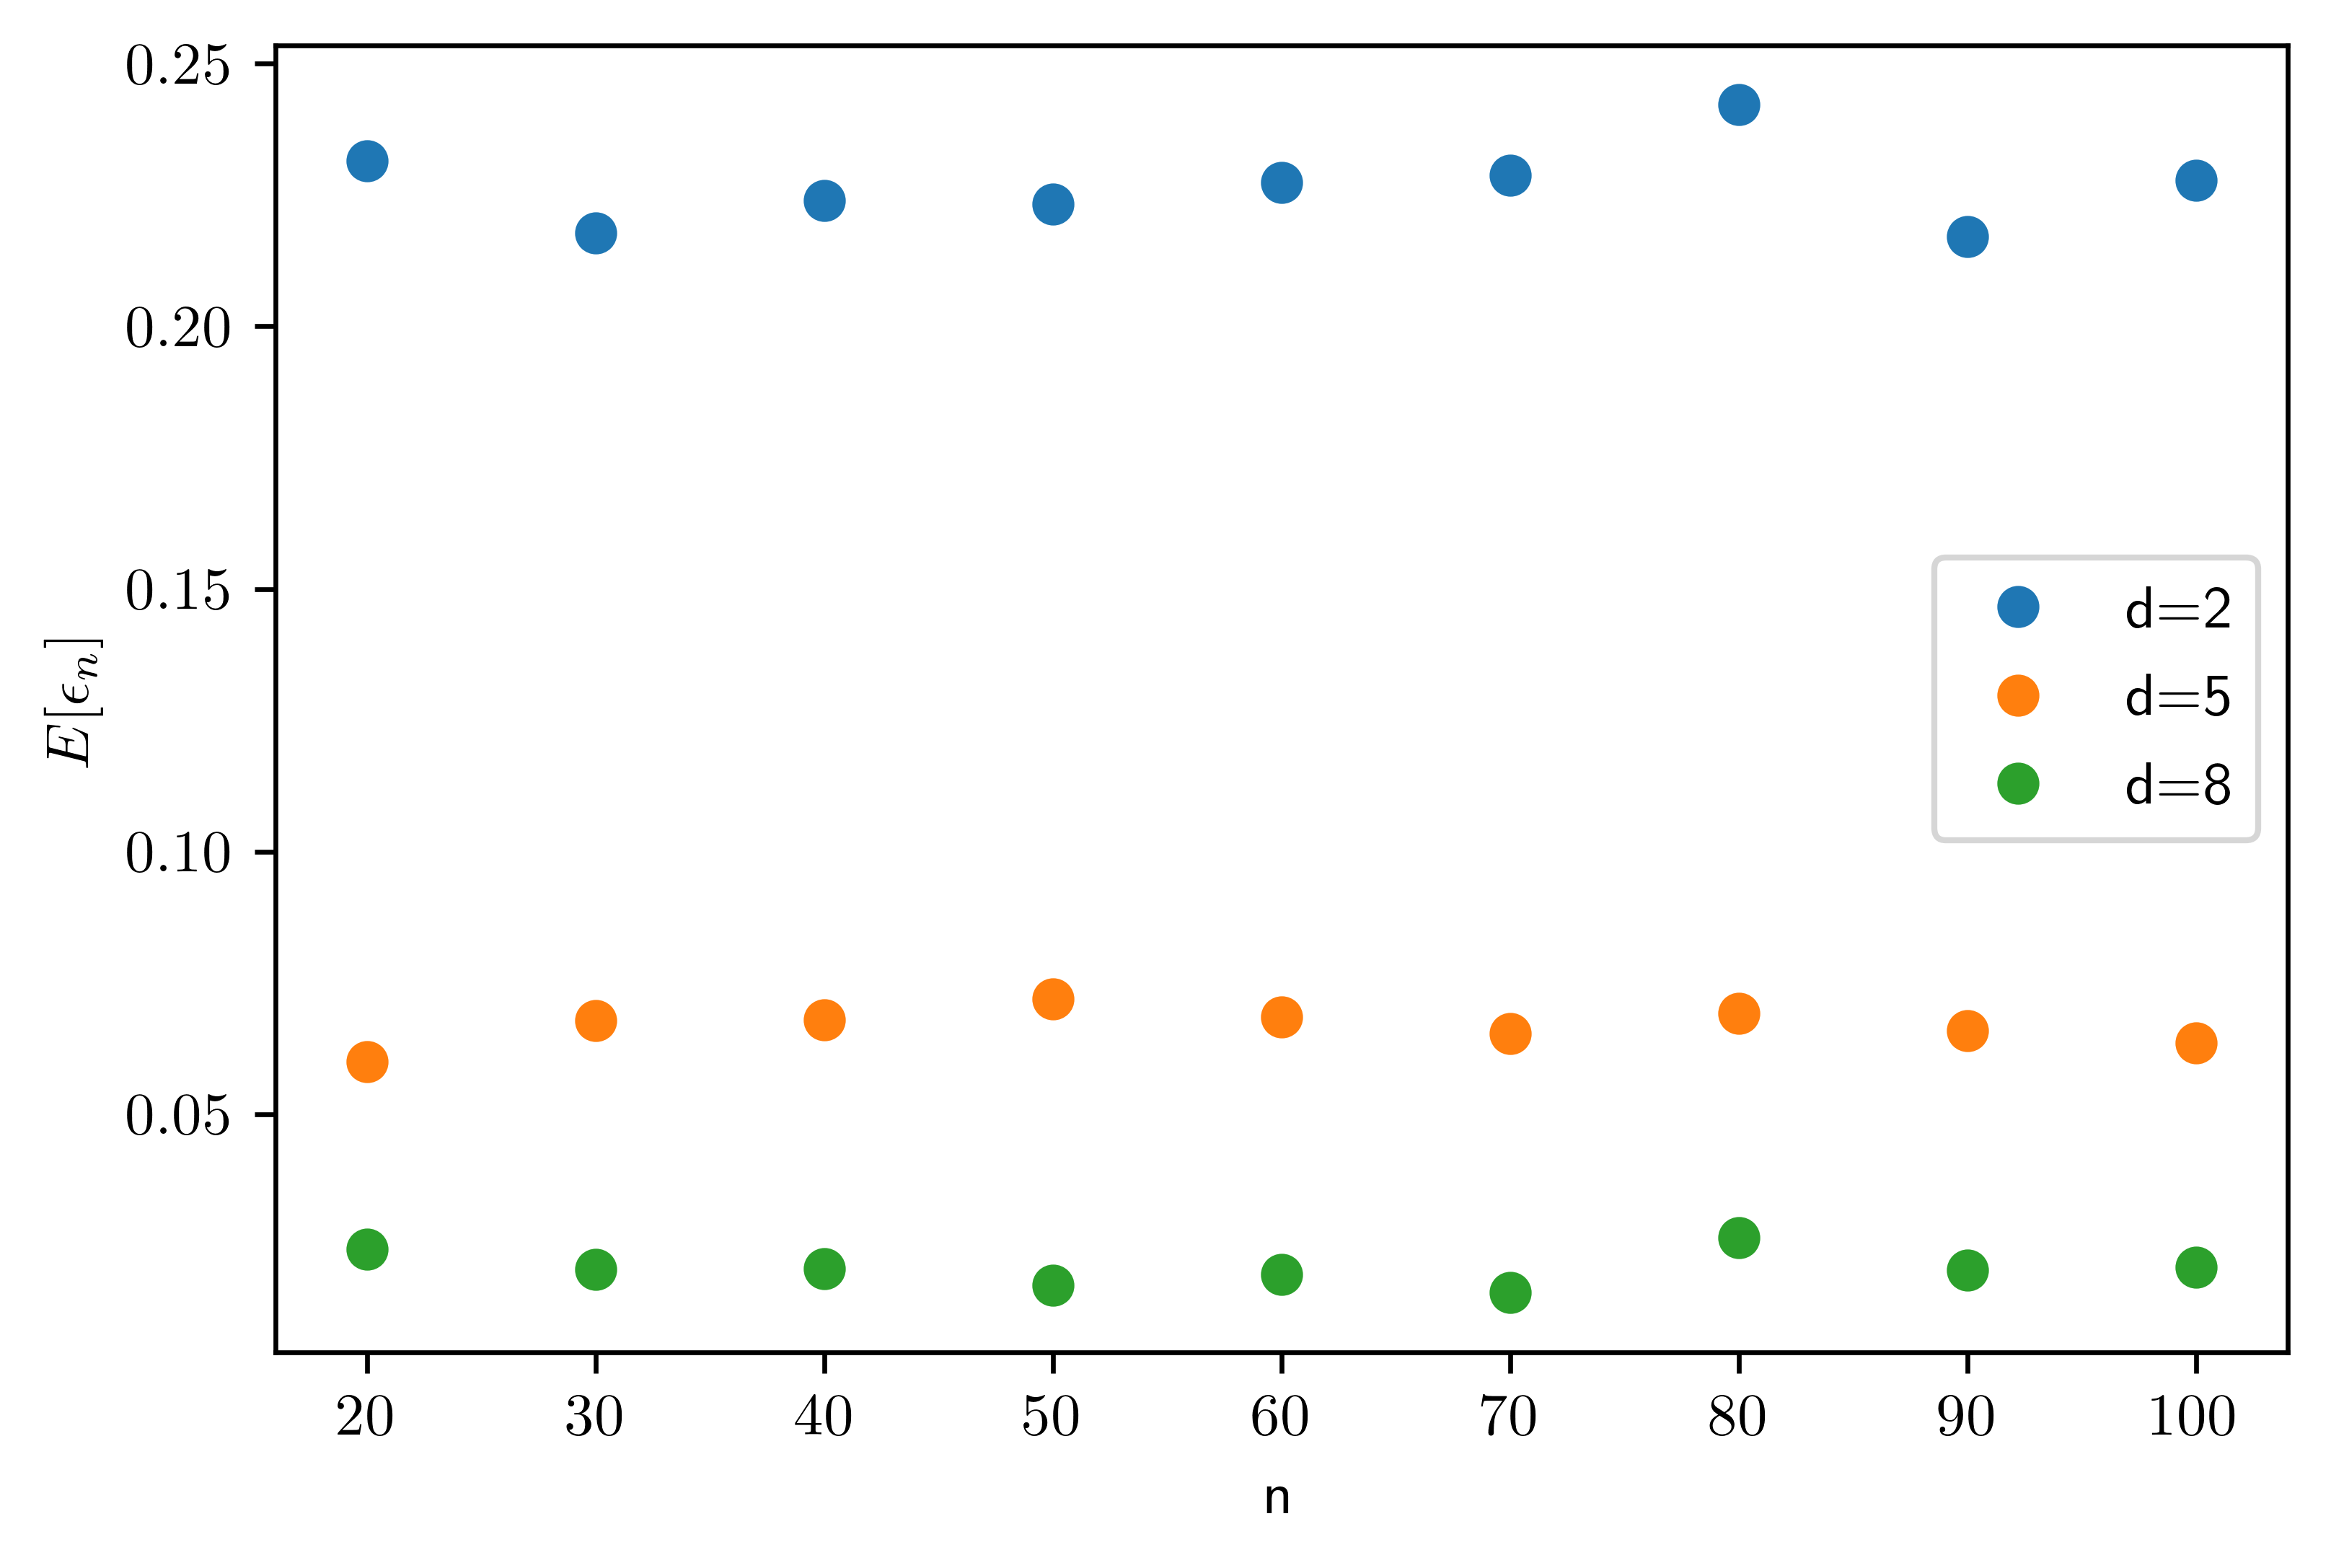
\includegraphics{hw2_files/figure-pdf/cell-4-output-1.pdf}

}

\end{figure}

\hypertarget{problem-4.2}{%
\subsection{Problem 4.2}\label{problem-4.2}}

\begin{quote}
A common method to extend binary classification rules to \(K\) classes,
\(K>2\), is the \emph{one-vs-one approach}, in which \(K(K-1)\)
classifiers are trained between all pairs of classes, and a majority
vote of assigned labels is taken.
\end{quote}

\hypertarget{sec-42a}{%
\subsubsection{(a)}\label{sec-42a}}

\begin{quote}
Formulate a multiclass version of parametric plug-in classification
using the one-vs-one approach.
\end{quote}

Let \(\psi^{*}_{i,j}\) be a one-one classifiers that \(i\neq j\), and
\(\{(i,j)| i\in [1,k], j \in [1,k], i\neq j\}\). For \(K\) classes,
there are \(K(K-1)\) classifiers; for each classifier \(\psi^{*}_{i,j}\)
and \(x\in R^d\),

\begin{equation}
    \psi^{*}_{ij,n} = 
    \begin{cases}
        1, & D_{ij, n}(x) > k_{ij,n}\\ 
        0, & \text{otherwise}
    \end{cases}
\end{equation}

where

\begin{itemize}
\tightlist
\item
  \(D_{ij,n}(x) = \ln \frac{p(x|\theta_{i,n})}{p(x|\theta_{j,n})}\)
\item
  \(k_{ij,n} = \ln\frac{P(Y=j)}{P(Y=i)}\)
\item
  Noted that feature-label distribution is expressed via a familty of
  PDF \(\{p(x|\theta_i) | \theta \in \Theta \subseteq R^m\}\), for
  \(i=1,\dots,K\).
\end{itemize}

Let \(\psi^{*}_{i,n} = \sum_{j\neq i} I_{\psi^{*}_{ij,n}=1}\), and the
one-vs-one classifier is

\[\psi^{*}_{n}(x) = \arg\max_{k=1,\dots,K} \psi^{*}_{k,n}\]

\hypertarget{sec-42b}{%
\subsubsection{(b)}\label{sec-42b}}

\begin{quote}
Show that if the threshold \(k_{ij,n}\) between classes \(i\) and \(j\)
is given by \(\frac{\ln\hat{c}_j}{\ln\hat{c}_i}\), then the one-vs-one
parametric classification rule is equivalent to the simple decision.
\[\psi_{n}(x) = \arg\max_{k=1,...,K} \hat{c}_{k} p(x|\theta_{k,n}), x\in R^d\]
(For simplicity, you may ignore the possibility of ties.)
\end{quote}

\hypertarget{c}{%
\subsubsection{(c)}\label{c}}

\begin{quote}
Applying the approach in items \protect\hyperlink{sec-42a}{(a)} and
\protect\hyperlink{sec-42b}{(b)}, formulate a multiclass version of
Gaussian discriminant analysis. In the case of multiclass NMC, with all
thresholds equal to zero, how does the decision boundary look like?
\end{quote}

\hypertarget{problem-4.3}{%
\subsection{Problem 4.3}\label{problem-4.3}}

\begin{quote}
Under the general Gaussian model
\(p(x|Y=0)\sim \mathcal{N}_d(\mu_0, \sum_0)\) and
\(p(x|Y=1)\sim \mathcal{N}_d(\mu_1, \sum_1)\), the classification error
\(\epsilon_n = P(\psi_n(X)\neq Y| S_n)\) of \emph{any} linear classifier
in the form

\begin{equation}
   \psi_{n}(x) = 
   \begin{cases}
       1,& a_{n}^{T}x + b_n > 0,\\ 
       0,& \text{otherwise}
   \end{cases}
\end{equation}

(examples discussed so far include LDA and its variants, and the
logistic classifier) can be readily computed in terms of \(\Phi\) (the
CDF of a standard normal random variable), the classifier parameters
\(a_n\) and \(b_n\), and the distributional parameters \(c=P(Y=1)\),
\(\mu_0\), \(\mu_1\), \(\Sigma_0\), and \(\Sigma_1\).
\end{quote}

\hypertarget{a}{%
\subsubsection{(a)}\label{a}}

\begin{quote}
Show that

\[\epsilon_n = (1-c)\Phi\left( \frac{a_{n}^{T}\mu_0 + b_n}{\sqrt{a_{n}^{T}\Sigma_0 a_n}} \right) + c \Phi\left( -\frac{a^{T}_{n}\mu_1 + b_n}{\sqrt{a_{n}^{T}\Sigma_1 a_n}}\right)\]

Hint: the discriminant \(a^{T}_{n}x+b_n\) has a simple Gaussian
distribution in each class.
\end{quote}

\hypertarget{b}{%
\subsubsection{(b)}\label{b}}

\begin{quote}
Compute the errors of the NMC, LDA, and DLDA classifiers in Example 4.2
if \(c=1/2\), \begin{equation*}
\mu_0 =
\begin{bmatrix}
2\\ 
3
\end{bmatrix},
\mu1 =
\begin{bmatrix}
6\\ 
5
\end{bmatrix},
\Sigma_0 = 
\begin{bmatrix}
1 & 1\\ 
1 & 2
\end{bmatrix},
\text{ and } 
\Sigma_1 = 
\begin{bmatrix}
4 & 0\\
0 & 1
\end{bmatrix}
\end{equation*} Which classifier does the best?
\end{quote}

\hypertarget{problem-4.4}{%
\subsection{Problem 4.4}\label{problem-4.4}}

\begin{quote}
Even in the Gaussian case, the classification error of quadratic
classifiers in general require numerical integration for its
computation. In some special simple cases, however, it is possible to
obtain exact solutions. Assume a two-dimensional Gaussian problem with
\(P(Y=1)=\frac{1}{2}\), \(\mu_0=\mu_1 = 0\),
\(\Sigma_0=\sigma_{0}^{2}I_2\), and \(\Sigma_1 = \sigma^{2}_{1}I_2\).
For definiteness, assume that \(\sigma_0 < \sigma_1\).
\end{quote}

\hypertarget{a-1}{%
\subsubsection{(a)}\label{a-1}}

\begin{quote}
Show that the Bayes classifier is given by \begin{equation}
\psi^{*}(x) = 
\begin{cases}
1, &\|x\| > r^{*},\\
0, &\text{ otherwise },
\end{cases}
\quad \text{ where } r^{*} = \sqrt{2\left(\frac{1}{\sigma_{0}^{2}} - \frac{1}{\sigma_{1}^{2}}\right)^{-1}\ln\frac{\sigma^{2}_{1}}{\sigma^{2}_{0}}}
\end{equation} In particular, the optimal decision boundary is a circle
of radius \(r^{*}\).
\end{quote}

The inverted \(\Sigma_1\) and \(\Sigma_2\) are\footnote{\begin{equation}\begin{bmatrix}
  a & b\\ 
  c & d
  \end{bmatrix}^{-1} = \frac{1}{ad-bc}\begin{bmatrix}
  d & -b\\ 
  -c & a
  \end{bmatrix}
  \end{equation}}

\begin{align}
    \Sigma_0 &= \sigma_{0}^2 I_2 = \begin{bmatrix}
        \sigma_{0}^2 & 0 \\
        0 & \sigma_{0}^2
    \end{bmatrix}\\ 
    \Sigma_{0}^{-1} &= \frac{1}{\sigma_{0}^{4}} \begin{bmatrix}
        \sigma_{0}^2 & 0 \\
        0 & \sigma_{0}^2
    \end{bmatrix} = \sigma_{0}^{-2}\begin{bmatrix}
            1 & 0\\
            0 & 1
        \end{bmatrix} = \sigma^{-2}_{0}I_2\\
    \Sigma^{-1}_{1} &= \sigma^{-2}_{1}I_2
\end{align}

Use the derivation in Braga-Neto (2020, 74),

\begin{equation}
    A_n = \begin{bmatrix}
        a_{11} & a_{12}\\ 
        a_{12} & a_{22}
    \end{bmatrix} = \frac{-1}{2} \Sigma_{1}^{-1} - \Sigma_{0}^{-1} = \frac{-1}{2}(\sigma_{1}^{-2} - \sigma_{0}^{-2}) \begin{bmatrix}
        1 & 0\\ 
        0 & 1
    \end{bmatrix}
\end{equation}

\begin{align}
    b_n &= \begin{bmatrix}
        b_{n,1}\\ 
        b_{n,2}
    \end{bmatrix}
    = \Sigma_{1}^{-1}\underbrace{\mu_1}_{=0} - \Sigma_{0}^{-1}\underbrace{\mu_{0}}_{=0}\\
        &= \begin{bmatrix}
            0\\ 
            0
        \end{bmatrix}
\end{align}

\[c = -\frac{1}{2}\ln\frac{|\Sigma_1|}{|\Sigma_0|} = \frac{-1}{2}\ln\frac{\sigma_{1}^{4}}{\sigma_{0}^{4}} = -\ln \frac{\sigma_{1}^2}{\sigma_{0}^2}\]

According to Braga-Neto (2020, Eq. 4.26), the 2-dimensional QDA decision
boundary is

\begin{align}
    D(x) = a_{11}x^{2}_1 + 2 a_{12}x_1x_2 + a_{22}x^{2}_{2} + b_1 x_1 + b_2 x_2 + c &= 0\\
    a_{11}(x_{1}^{2} + x_{2}^{2}) &= \ln \frac{\sigma_{1}^2}{\sigma_{0}^2}\\
    x^{2}_{1} + x^{2}_{2} &= 2(\frac{1}{\sigma^{2}_{0}} - \frac{1}{\sigma^{2}_{1}})^{-1}\ln\frac{\sigma_{1}^2}{\sigma_{0}^2}\\
    r^{*} = \sqrt{x^{2}_{1} + x^{2}_{2}} &= \sqrt{2(\frac{1}{\sigma^{2}_{0}} - \frac{1}{\sigma^{2}_{1}})^{-1}\ln\frac{\sigma_{1}^2}{\sigma_{0}^2}}
\end{align}

Noted that
\(\left(\frac{1}{\sigma^{2}_{0}} - \frac{1}{\sigma^{2}_{1}}\right) > 0\)
because \(\sigma_0 < \sigma_1\)

For any point \(\|x_j\| > r^{*}\), the discriminant (\(D\)) is larger
than \(0\), and \(\psi^{*}(x_j) = 1\).

\hypertarget{b-1}{%
\subsubsection{(b)}\label{b-1}}

\begin{quote}
Show that the corresponding Bayes error is given by
\[\epsilon^{*} = \frac{1}{2} - \frac{1}{2}(\frac{\sigma^{2}_{1}}{\sigma^{2}_{0}} - 1)e^{-(1-\frac{\sigma^{2}_{0}}{\sigma^{2}_{1}})^{-1}\ln \frac{\sigma^{2}_{1}}{\sigma^{2}_{0}}}\]
In particular, the Bayes error is a function only of the ratio of
variances \(\frac{\sigma^{2}_{1}}{\sigma^{2}_{0}}\), and
\(\epsilon^{*}\rightarrow 0\) as
\(\frac{\sigma^{2}_{1}}{\sigma^{2}_{0}} \rightarrow \infty\).

Hint: use polar coordinates to solve the required integrals
analytically.
\end{quote}

\begin{align}
    \epsilon^{0}[\psi^{*}] 
    &= P(D^{*}(X)>k^{*}|Y=0)\\ 
    &= P(\|x\|>r^{*} | Y=0)
\end{align}

\begin{align}
    \epsilon^{0}[\psi^{*}] 
    &= P(D^{*}(X)\leq k^{*}|Y=1)\\ 
    &= P(\|x\|\leq r^{*} | Y=1)
\end{align}

\begin{verbatim}
- WIP
-  https://ardianumam.wordpress.com/2017/10/19/deriving-gaussian-distribution/
- Integrate the area outside the circle with (Y=0) and Integrate the area inside the circle with (Y=1)
\end{verbatim}

\hypertarget{c-1}{%
\subsubsection{(c)}\label{c-1}}

\begin{quote}
Compare the optimal classifier to the QDA classifier in Example 4.3.
Compute the error of the QDA classifier and compare to the Bayes error.
\end{quote}

\hypertarget{problem-4.8-python-assignment}{%
\subsection{Problem 4.8 (Python
Assignment)}\label{problem-4.8-python-assignment}}

\begin{quote}
Apply linear discriminant analysis to the stacking fault energy (SFE)
dataset (see Braga-Neto (2020, sec. A8.4)), already mentioned in
Braga-Neto (2020, ch.~1). Categorize the SFE values into two classes,
low (SFE \(\leq 35\)) and high (SFE \(\geq 45\)), excluding the middle
values.
\end{quote}

\hypertarget{a-2}{%
\subsubsection{(a)}\label{a-2}}

\begin{quote}
Apply the preprocessing steps in \texttt{c01\_matex.py} to obtain a data
matrix of dimensions
\(123 (\text{number of sample points}) \times 7 (\text{number of features})\),
as described in Braga-Neto (2020, sec. 1.8.2). Define low (SFE
\(\leq 35\)) and high (SFE \(\geq 45\)) labels for the data. Pick the
first \(20\%\) of the sampe point s to be the training data and the
remaining \(80\%\) to be test data.
\end{quote}

\hypertarget{b-2}{%
\subsubsection{(b)}\label{b-2}}

\begin{quote}
Using the function \texttt{ttest\_ind} from the \texttt{scipy.stats}
module, apply Welch's two-sample t-test on the training data, and
produce a table with the predictors, \emph{T} statistic, and
\emph{p}-value, ordered with largest absolute \emph{T} statistics at the
top.
\end{quote}

\hypertarget{c-2}{%
\subsubsection{(c)}\label{c-2}}

\begin{quote}
Pick the top two predictors and design an LDA classifier. (This is an
example of \emph{filter feature selection}, to be discussed in Chapter
9.). Plot the training data with the superimposed LDA decision boundary.
Plot the testing data with the superimposed previously-obtained LDA
decision boundary. Estimate the classification error rate on the
training and test data. What do you observe?
\end{quote}

\hypertarget{d}{%
\subsubsection{(d)}\label{d}}

\begin{quote}
Repeat for the top three, and five predictors. Estimate the errors on
the training and testing data (there is no need to plot the
classifiers). What can you observe?
\end{quote}

\hypertarget{references}{%
\subsection{References}\label{references}}

\hypertarget{appendix}{%
\subsection{Appendix}\label{appendix}}

\hypertarget{question-about-probelm-4.2b}{%
\subsubsection{Question about Probelm
4.2b}\label{question-about-probelm-4.2b}}

\begin{verbatim}
[Question][Problem 4.2(b)]
The treshold `k_{ij,n}` is given by `\frac{\ln \hat{c}_j}{\hat{c}_i}`. However, this setting is different from the text book (P. 68), that is `k=\ln \frac{c_0}{c_1}`. 

Is this a typo or intenionally assigned?
\end{verbatim}

\begin{longtable}[]{@{}
  >{\raggedright\arraybackslash}p{(\columnwidth - 2\tabcolsep) * \real{0.5000}}
  >{\raggedright\arraybackslash}p{(\columnwidth - 2\tabcolsep) * \real{0.5000}}@{}}
\toprule()
\begin{minipage}[b]{\linewidth}\raggedright
Textbook p.68
\end{minipage} & \begin{minipage}[b]{\linewidth}\raggedright
Problem 4.2 (b)
\end{minipage} \\
\midrule()
\endhead
\(k^{*}=\ln\frac{c_0}{c_1}\) &
\(k_{ij,n}=\frac{\ln\hat{c_j}}{\ln \hat{c}_i}\) \\
\bottomrule()
\end{longtable}

\begin{tcolorbox}[enhanced jigsaw, titlerule=0mm, breakable, arc=.35mm, bottomtitle=1mm, coltitle=black, leftrule=.75mm, colbacktitle=quarto-callout-tip-color!10!white, colframe=quarto-callout-tip-color-frame, opacitybacktitle=0.6, toptitle=1mm, left=2mm, title=\textcolor{quarto-callout-tip-color}{\faLightbulb}\hspace{0.5em}{Tip}, rightrule=.15mm, bottomrule=.15mm, toprule=.15mm, colback=white, opacityback=0]
dwf
\end{tcolorbox}

\hypertarget{refs}{}
\begin{CSLReferences}{1}{0}
\leavevmode\vadjust pre{\hypertarget{ref-braga2020fundamentals}{}}%
Braga-Neto, Ulisses. 2020. \emph{Fundamentals of Pattern Recognition and
Machine Learning}. Springer.

\end{CSLReferences}



\end{document}
